\section{Detalles de la propuesta}
En este apartado, se dará una visión global del contenido y funcionamiento de nuestra propuesta.
Se realizará una descripción completa de nuestro enfoque, desde los conceptos de IA
empleados hasta las herramientas y tecnologías empleadas para su resolución. En primer lugar, se
detalla cómo se ha realizado la generación de los modelos, los tipos utilizados y sus
características, así como cualquier concepto relacionado. Posteriormente, se describen las
técnicas empleadas para evaluar el rendimiento de los modelos. Continuaremos con la explicación
en detalle de las \textit{features} empleadas, qué representan y cómo se ha realizado su cálculo.
Finalmente, procederemos a explicar detalles técnicos de la implementación, como las tecnologías
y recursos empleados, el procedimiento de extracción de datos, el entorno de ejecución, etc. En
los siguientes apartados se describe con detalle cada uno de estos puntos.

\subsection{Construcción del modelo} \label{sec:model_construction}

El Aprendizaje Automático (\textit{Machine Learning}, ML)
es un campo de la Inteligencia Artificial que se centra en desarrollar algoritmos y modelos que
sean capaces de aprender y mejorar su desempeño en tareas específicas a partir de datos, sin la
necesidad de ser explícitamente programadas. Los sistemas de ML identifican patrones en
los datos y utilizan estos patrones para hacer predicciones o tomar decisiones sobre los datos.
Podemos encontrarnos con dos tipos de aprendizaje automático:

\begin{itemize}
	\item \textbf{Supervisado}: en este tipo de aprendizaje el modelo es entrenado utilizando un
    conjunto de datos etiquetados. En este contexto ``etiquetado'' significa que cada instancia
    en el conjunto de datos viene con una entrada (conjunto de características) y una salida
    conocida (etiqueta o valor objetivo). En nuestro problema, la entrada sería el conjunto de
    características (\textit{features}) que vamos a usar y, la salida, el resultado de la
    integración continua (exitosa o fallida).
	\item \textbf{No supervisado}: en este tipo de aprendizaje el modelo es entrenado utilizando
    un conjunto de datos que no tiene etiquetas ni salidas predefinidas. A diferencia del
    supervisado, en el que se indica al modelo lo que debe predecir, en el no supervisado el
    modelo explora los datos en busca de patrones, estructuras, o relaciones ocultas.
\end{itemize}

Teniendo esto en cuenta, nos encontramos claramente ante un problema de aprendizaje supervisado,
ya que tenemos las características propias de cada \textit{build}, que sería el conjunto de
entrada que proporcionamos al modelo y, por otro lado, los resultados de las ejecuciones, que
conformarían las etiquetas o valores objetivo de nuestro problema.\\

Para poder responder a la pregunta de investigación \textbf{PI-1}, debemos explorar los
distintos algoritmos de Aprendizaje Automático que existen y ver cuál de ellos ofrece mejores
resultados en el problema que nos ocupa. En nuestro caso, nos encontramos con un claro problema
de clasificación binaria en el ámbito del aprendizaje automático supervisado. En este contexto,
tenemos dos clases posibles:
\begin{enumerate}
    \item \textbf{Clase positiva} (fallo de la \textit{build}): predicción de que la \textit{build}
    fallará.\\
    \item \textbf{Clase negativa} (éxito de la \textit{build}): predicción de que la \textit{build}
    tendrá éxito.
\end{enumerate}

Por lo tanto, dado que nos encontramos con este tipo de problema, se ha decidido utilizar seis
algoritmos de clasificación supervisada, entre los que nos encontramos:

\begin{enumerate}
    \item \textbf{Árboles de Decisión (\textit{Decision Trees}, DT)}. Dividen el conjunto de datos
    en subconjuntos más pequeños y más simples, basándose en ciertas características o condiciones,
    que están representadas en un gráfico similar a un árbol. Cada nodo interno del árbol
    representa una característica (o atributo), y cada rama representa el resultado de la
    partición de los datos en función de esa característica. Las hojas del árbol contienen las
    etiquetas o valores objetivo.\\
    \item \textbf{Bosques Aleatorios (\textit{Random Forest}, RF)}. Es un algoritmo de aprendizaje
    supervisado que crea un conjunto de árboles de decisión durante el entrenamiento y realiza
    la predicción promediando las predicciones de cada árbol individual. Es una técnica de
    ensamblaje que combina múltiples modelos de aprendizaje para mejorar la precisión y la
    estabilidad del modelo.\\
    \item \textbf{Regresión Logística (\textit{Logistic Regression}, LR)}. Es un algoritmo de
    clasificación que se utiliza para predecir la probabilidad de que una variable dependiente
    pertenezca a una categoría particular. Aunque se llama regresión, en realidad es un algoritmo
    de clasificación binaria.\\
    \item \textbf{Máquinas de Soporte Vectorial (\textit{Support Vector Machines}, SVM)}. Es un
    algoritmo de clasificación que busca encontrar el hiperplano que mejor divide un conjunto de
    datos en dos clases. El hiperplano es la línea que maximiza el margen entre las dos clases. Si
    los datos no son linealmente separables, se puede utilizar un truco matemático llamado
    \textit{kernel trick} para transformar los datos en un espacio de mayor dimensión donde sí
    sean separables.\\
    \item \textbf{Vecinos más Cercanos (\textit{K-Nearest Neighbors}, KNN)}. Es un algoritmo de
    clasificación que se basa en la idea de que los puntos de datos que son similares deben
    pertenecer a la misma clase. Para predecir la clase de un nuevo punto de datos, el algoritmo
    busca los $k$ puntos de datos más cercanos en el conjunto de entrenamiento y asigna la clase
    más común entre esos vecinos.\\
    \item \textbf{Redes Neuronales (\textit{Neural Networks}, NN)}. Son un conjunto de algoritmos
    de aprendizaje automático que intentan imitar el funcionamiento del cerebro humano. Consiste en
    una red de nodos interconectados, llamados neuronas, que se organizan en capas. Está formada
    por una capa de entrada, una o varias capas ocultas y una capa de salida. Cada nodo está
    conectado a los demás y tiene su propia ponderación y umbral asociados. Concretamente, se ha
    utilizado un Perceptrón Multicapa, que es un tipo de red neuronal utilizado para tareas de
    clasificación. Cada neurona en un MLP se conecta a las de la capa anterior con pesos
    y aplica una función de activación a su suma ponderada.
\end{enumerate}

Para realizar la predicción, no únicamente se le proporciona al modelo el conjunto de
características de la \textit{build} y se predice, si no que se sigue un procedimiento más
complejo y que simula el funcionamiento de SmartBuildSkip \cite{2}. Para comprenderlo, veamos
el siguiente pseudocódigo:

\begin{algorithm}[H]
    \caption{\textit{SmartBuildSkip con nuestra implementación}}
    \begin{algorithmic}[1]
    \State \textbf{Input:} List of builds
    \State \textbf{Output:} Predictions of builds outcomes
    
    \State in\_failure\_sequence $\gets$ False \Comment{Inicializar estado de secuencia de fallos}
    \For {each build in builds}
        \If{in\_failure\_sequence}
            \State Prediction $\gets$ Fail  \Comment{Predicción automática de fallo}
            \If{build passes}               \Comment{Comprobar resultado}
                \State in\_failure\_sequence $\gets$ False \Comment{Error en la predicción, vuelve a predecir con ML}
            \EndIf
            \Else
            \State Prediction $\gets$ Machine Learning Prediction \Comment{Predicción usando ML}
            \If {Prediction = Pass}
                \State Accumulate changes with next build       \Comment{Se salta la build, acumulando cambios}
            \Else
                \If{build fails}                                \Comment{Comprobar resultado}
                    \State in\_failure\_sequence $\gets$ True   \Comment{Entra en predicción automática de fallo}
                \EndIf
            \EndIf
        \EndIf
    \EndFor
    \end{algorithmic}
\end{algorithm}

Como podemos observar, este algoritmo se divide en dos partes: una en la que predice
automáticamente que la \textit{build} fallará y otra en la que se realiza la predicción mediante
el uso de un modelo de aprendizaje automático. Esta forma de proceder es debida a las dos
hipótesis que comentamos en la Sección \ref{sec:related_work}, que muchas \textit{builds} fallan
consecutivamente después de que otra haya fallado y que las \textit{builds} exitosas siempre son
más numerosas que las fallidas. Esto hace que nuestro algoritmo pueda saltarse mayor número de
\textit{builds} a la vez que captura una mayor cantidad de \textit{build failures}.
Consecuentemente, debido a la no ejecución de estas \textit{builds}, se estará logrando una
optimización de recursos computacionales.

\subsubsection{Hiperparámetros.}
Cuando se define un algoritmo de clasificación, es importante seleccionar y ajustar con cuidado
los hiperparámetros, ya que estos controlan aspectos clave del proceso de entrenamiento y pueden
determinar la capacidad del modelo para generalizar a nuevos datos. Para la definición de nuestros
algoritmos de clasificación, se ha utilizado la biblioteca \textit{scikit-learn}, una popular
biblioteca de \textit{Python} para \textit{Machine Learning} y análisis de datos. Por lo general,
se han definido todos los algoritmos con los parámetros por defecto de la biblioteca
\textit{scikit-learn}, con las siguientes particularidades:

\begin{itemize}
	\item En un conjunto de datos que contiene \textit{builds}, donde el número de \textit{builds}
    exitosas es mucho mayor que el de \textit{builds} fallidas, estamos ante un problema de
    desequilibrio de clases. En este contexto, asignar distintos pesos a las clases es una
    estrategia útil para entrenar un modelo que sea más sensible en la detección de
    \textit{builds failures}, a pesar de ser poco numerosas. Para ello, se ha definido un peso de
    20:1 a favor de las \textit{build failures} en Árbol de Decisión, Bosque Aleatorio, Regresión
    Logística y Máquinas de Soporte Vectorial.\\

	\item En Regresión Logística, se establece el número máximo de iteraciones que el algoritmo de
    optimización realizará antes de detenerse. En este caso se utiliza el valor $15000$ para
    asegurar que el algoritmo tenga suficiente tiempo para converger.\\

	\item En el algoritmo de Máquinas de Soporte Vectorial, hemos añadido el hiperparámetro que
    habilita el cálculo de probabilidades de pertenencia a cada clase. Cuando el parámetro
    \textit{probability} está habilitado, el modelo ajusta de manera interna un modelo de
    probabilidad, permitiendo que las salidas del modelo sean las etiquetas de clase y sus
    probabilidades.\\

	\item Para el Perceptrón Multicapa (redes neuronales), se ha añadido, al igual que en Regresión
    Logística, un parámetro que indica el número máximo de iteraciones para entrenar la red
    neuronal. En este caso, se ha añadido con un valor de $15000$.
\end{itemize}

Además de los parámetros antes mencionados, todos ellos tienen definida la semilla de
reproducibilidad, que garantiza que los resultados sean reproducibles.

\subsection{Evaluación del modelo}
La evaluación de los modelos de clasificación tiene como objetivo medir y analizar el rendimiento
de los modelos en la tarea de clasificación. Esta evaluación permite identificar con qué precisión
el modelo puede predecir o clasificar nuevas instancias no vistas anteriormente, es decir, basándose
en un conjunto de datos de prueba. Para realizar la evaluación de los modelos en nuestro problema,
hemos seguido los siguientes pasos:

\begin{enumerate}
    \item \textbf{División del conjunto de datos}: se divide el conjunto de datos, en este caso
    \textit{features} de cada \textit{build}, en dos partes: el conjunto de entrenamiento y el
    conjunto de prueba. El conjunto de entrenamiento se utiliza para entrenar el modelo, mientras
    que el conjunto de prueba se usa para evaluar su rendimiento. Dada la naturaleza de nuestro
    problema, no podemos hacer esta división de manera aleatoria, ya que las \textit{builds} están
    relacionadas temporalmente entre sí, por lo que no sería realista realizar una predicción
    sobre una instancia antigua basándonos en \textit{builds} que se hayan ejecutado recientemente.
    Por lo tanto, en nuestro caso se ha dividido el conjunto de datos igualmente en dos partes,
    pero siendo el conjunto de entrenamiento más antiguo en su conjunto que el conjunto de prueba,
    que es más reciente. Por ejemplo, si se dividen los datos de entrenamiento y test en un 80\% y
    20\% respectivamente, el conjunto de entrenamiento contendrá el 80\% de las \textit{builds}
    más antiguas, mientras que el de prueba contendrá el 20\% de \textit{builds} más reciente.\\
    \item \textbf{Predicción}: una vez entrenado el modelo con el conjunto de entrenamiento, se
    realizan predicciones sobre el conjunto de prueba. Gracias a estas predicciones, podremos
    verificar si nuestros modelos se comportan bien frente a instancias nuevas o no vistas con
    anterioridad.\\
    \item \textbf{Métricas de evaluación}: una vez realizadas las predicciones, hemos definido
    las métricas de evaluación, que nos ayudarán a determinar el rendimiento de nuestros modelos.
    Las métricas que hemos usado son: \textit{accuracy}, \textit{precision}, \textit{recall},
    \textit{F1-score}, \textit{confusion matrix} y \textit{ROC curve}. Todas
    ellas han sido descritas en la Sección \ref{sec:research_questions}, exceptuando el área
    bajo la curva \textit{ROC} (\textit{Area Under the Curve, AUC}), que mide la capacidad de
    un modelo para distinguir entre clases positivas y negativas. Cuanto mayor sea el valor de
    \textit{AUC}, mejor será el desempeño del modelo en la clasificación, ya que esta indica una
    mayor capacidad para separar correctamente las clases.
\end{enumerate}

\subsubsection{Validación Cruzada.}
La validación cruzada (\textit{cross-validation}) es una técnica utilizada para la evaluación y
selección de modelos, midiendo su rendimiento y capacidad de generalización. Su objetivo
principal es evitar el sobreajuste (\textit{overfitting}), que ocurre cuando un modelo
aprende demasiado de los datos de entrenamiento y es incapaz de generalizar a nuevos datos. Esta
consiste en dividir el conjunto de datos en $k$ subconjuntos (\textit{folds}), entrenar el modelo
en $k-1$ subconjuntos y evaluarlo en el subconjunto restante. Este proceso se repite $k$ veces,
de forma que cada subconjunto se utiliza una vez como conjunto de prueba. Al final, se promedian
los resultados de las $k$ iteraciones para obtener una estimación más precisa del rendimiento del
modelo.\\

En nuestro caso particular, hemos tenido que hacer una ligera variación de esta técnica. En
nuestro problema, la división del conjunto de datos en $k$ subconjuntos no puede realizarse de
manera aleatoria, ya que no tendría sentido realizar predicciones para instancias más antiguas
utilizando para el entrenamiento instancias más recientes. Es decir, en nuestro problema existe
una dependencia temporal y, por tanto, la secuencia y el orden de los datos son críticos para la
validez de las predicciones. Los resultados y características de las \textit{builds} están
influenciados por las \textit{builds} anteriores. Esto se debe a que cada \textit{build} puede
depender de cambios de código, configuraciones y otros factores que se acumulen o evolucionen
con el tiempo. Por lo tanto, si se permite que las \textit{builds} más antiguas predigan utilizando
información de \textit{builds} más recientes, se introduciría un sesgo temporal que no reflejaría
el comportamiento real del sistema. Además de esto, usar datos de \textit{builds} futuras para
predecir \textit{builds} antiguas no solamente introduce un sesgo, si no que también puede dar
una falsa impresión de precisión del modelo, llevando a resultados artificialmente inflados de
precisión durante esta fase de evaluación.\\

En nuestra implementación dividimos el conjunto en 11 partes de forma secuencial, de modo que el
primer subconjunto contenga las \textit{builds} más antiguas y el último las \textit{builds} más
recientes. El subconjunto de \textit{folds} se recorre y en cada iteración, se entrena con la
acumulación de subconjuntos anteriores, y se evalúa con el siguiente subconjunto, dejando el resto
de subconjuntos sin utilizar. Siempre que se tengan $k$ \textit{folds} se realizarán $k-1$
iteraciones, ya que en la última iteración se utilizará el último subconjunto como conjunto de
prueba. Finalmente, dado que se habrán obtenido 10 resultados de las métricas de evaluación, se
promedian para obtener una estimación más precisa del rendimiento del modelo.\\

A continuación, se presenta de forma gráfica el funcionamiento de nuestro algoritmo de
\textit{key-fold cross validation}:

\begin{figure}[H]
    \centering
    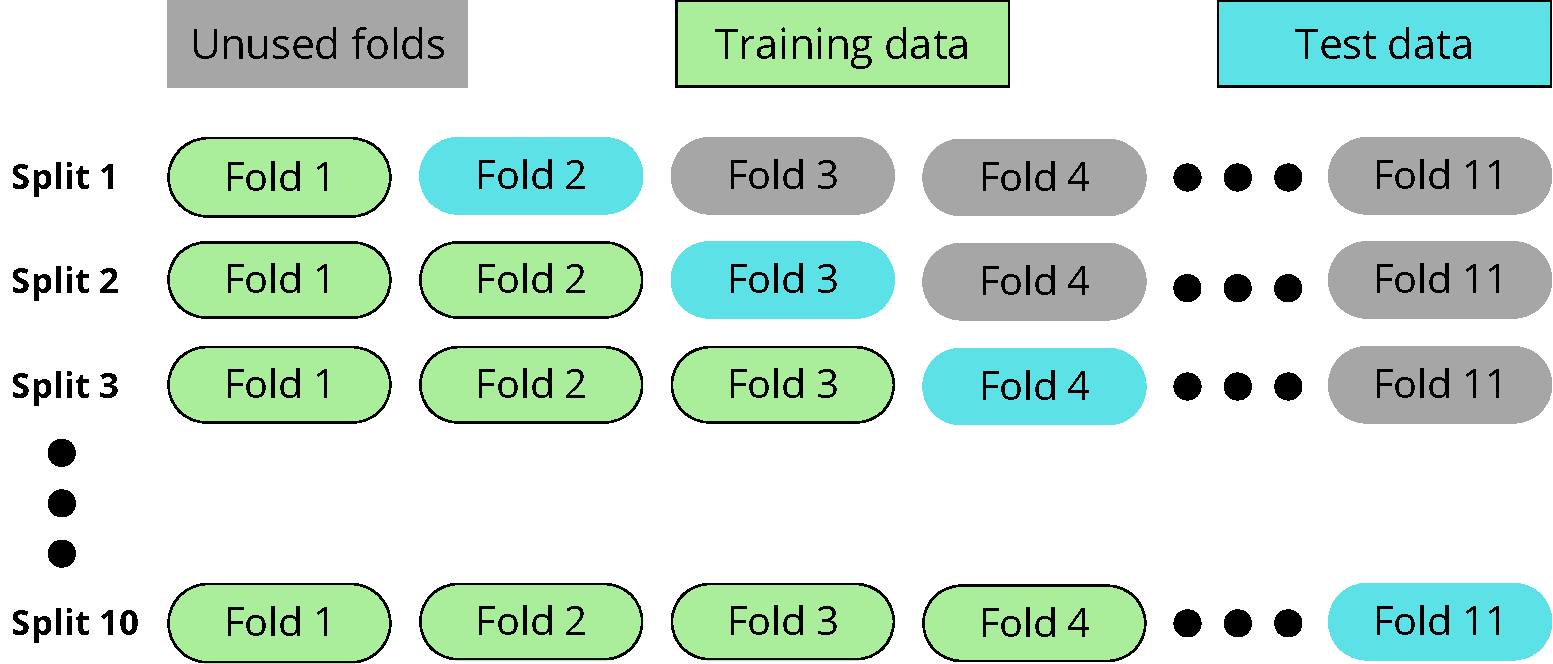
\includegraphics[scale=0.5]{images/Cross validation.pdf}
    \caption{Funcionamiento de la técnica \textit{key-fold cross validation}.}
    \label{fig:confusion_matrix}
\end{figure}

\subsubsection{Umbral de decisión.}
La evaluación de los modelos a distintos grados de sensibilidad es especialmente relevante cuando
se consideran problemas de clasificación con clases desbalanceadas o cuando el costo de los
errores varía entre clases. En el problema que nos ocupa, se dan ambas condiciones: por lo
general, el número de \textit{builds} exitosas es muy superior al de \textit{builds} fallidas y,
el costo de predecir un falso negativo no es el mismo que el de predecir un falso positivo. Al
ajustar la sensibilidad del modelo, se balancean las tasas de verdaderos positivos
(\textit{recall}) y falsos positivos, lo que permite optimizar el rendimiento del modelo para
diferentes contextos y necesidades. El hecho de variar el umbral de decisión permite al
desarrollador decidir hasta qué punto está dispuesto a obtener falsos positivos en las
predicciones. Por ejemplo, si se asigna un umbral de decisión bajo, se aumentarán las tasas de
verdaderos positivos, pero también aumentará el número de falsos positivos, es decir, el algoritmo
predecirá un mayor número de veces que la \textit{build} falla, haciendo al desarrollador ejecutar
\textit{builds} que realmente no fallaban. Por otro lado, si se asigna un umbral de decisión más
conservador, se reducirán los falsos positivos, pero también con el riesgo de predecir alguna
\textit{build} como exitosa cuando realmente no lo es, teniendo el caso del falso negativo.\\


Muchos algoritmos de aprendizaje automático pueden predecir una probabilidad de
pertenencia a una clase. Esto es útil porque proporciona una medida de la certeza o incertidumbre
de una predicción y ofrece más detalles que solo predecir la etiqueta de la clase. En nuestro
problema, es necesario convertir estas probabilidades en el valor de una clase. Esta conversión
se basa en un parámetro llamado ``umbral de decisión''. El valor por defecto de este umbral
es $0.5$ para probabilidades normalizadas en el intervalo $[0, 1]$. Por ejemplo, dadas las
etiquetas de nuestro problema: $0$ (la \textit{build} falla) y $1$ (la \textit{build} pasa), si
la probabilidad de que una \textit{build} falle es igual o mayor a $0.5$, se predecirá que la
\textit{build} es exitosa, mientras que si es menor a $0.5$, se predecirá que la \textit{build}
falla.\\

En nuestra implementación, hemos evaluado el rendimiento de todos los modelos y variantes del
mismo para valores del umbral de decisión comprendidos en el intervalo $[0, 1]$. Para ello, se
han calculado las métricas de evaluación para cada valor del umbral y se han representado en
gráficos para poder comparar el rendimiento de los modelos en función del umbral de decisión. De
esta forma, se ha podido determinar cuál de los modelos es el que mejor rendimiento ofrece y cuál
de las implementaciones es la que mejor resultado proporciona.


\subsection{\textit{Features} empleadas}\label{sec:features_used}
Las \textit{features} o características son las propiedades o atributos que se utilizan como entrada
para entrenar un modelo. Son elementos fundamentales que permiten al modelo aprender patrones y
tomar decisiones basadas en los datos. Las \textit{features} recogen información relevante de
los datos, en este caso de las \textit{builds}. La calidad y relevancia de las mismas afecta
al rendimiento del modelo, por lo que escoger las adecuadas es fundamental. Al hacer la selección
de las \textit{features}, hay que tener en cuenta lo siguiente:

\begin{itemize}
    \item Elegir \textit{features} que sean relevantes y representativas del problema es importante
    para que el modelo sea preciso y eficiente. Además, ayuda a reducir la dimensionalidad
    del problema, lo que puede mejorar la eficiencia computacional y la interpretabilidad del
    modelo.\\
    \item Seleccionar gran cantidad de \textit{features} puede llevar a un sobreajuste del modelo,
    donde el modelo aprende de patrones de datos ruidosos o irrelevantes. Esto puede llevar a un
    rendimiento bajo y a modelos menos generalizables
\end{itemize}

\noindent A continuación, se presentan las features estudiadas en nuestro problema.

\begin{table}[H]
    \centering
    \caption{\textit{Build features}.}
    \label{tab:features}

    \begin{tabular}{|>{\centering\arraybackslash}m{3cm}|>{\centering\arraybackslash}m{4cm}|>{\centering\arraybackslash}m{7cm}|} % Encabezados centrados
        \hline
        \textbf{\textit{Clasificación}} &\textbf{\textit{Feature}} & \textbf{Descripción breve} \\
        \hline
    \end{tabular}
    \begin{tabular}{|>{\raggedright\arraybackslash}m{3cm}|>{\raggedright\arraybackslash}m{4cm}|>{\raggedright\arraybackslash}m{7cm}|} % Contenido alineado a la izquierda en la esquina superior
        \hline
        \multirow{4}{=}{Consideradas en SmartBuildSkip} & \textit{Number Commits} (NC) & El número de \textit{commits desde la última \textit{build}.} \\
        \cline{2-3}
        & \textit{Files Changed} (FC) & El número de archivos modificados desde la última \textit{build}, incluyendo archivos añadidos, modificados y eliminados.\\
        \cline{2-3}
        & \textit{Source Lines Changed} (LC) & El número de líneas de código modificadas desde la última \textit{build}, incluyendo líneas añadidas y eliminadas.\\
        \cline{2-3}
        & \textit{Test Lines Changed} (LT) & El número de líneas de código de \textit{test} modificadas desde la última \textit{build}, incluyendo líneas añadidas y eliminadas.\\
        \Xhline{1pt}
        \multirow{6}{=}{Consideradas en SmartBuildSkip pero no utilizadas} & \textit{Performance Short} (PS) & La proporción de \textit{builds} exitosas en las últimas cinco \textit{builds}.\\
        \cline{2-3}
        & \textit{Performance Long} (PL) & La proporción de \textit{builds} exitosas de todas las \textit{builds} previas.\\
        \cline{2-3}
        & \textit{Time Frequency} (TF) & El intervalo de tiempo en horas desde la última \textit{build}.\\
        \cline{2-3}
        & \textit{Failure Distance} (FD) & El número de \textit{builds} exitosas desde la última \textit{build} fallida.\\
        \cline{2-3}
        & \textit{Week Day} (WD) & El día de la semana en el que se ha ejecutado la \textit{build}.\\
        \cline{2-3}
        & \textit{Day Hour} (DH) & La hora del día en la que se ha ejecutado la \textit{build}.\\
        \Xhline{1pt}
        \multirow{7}{=}{Nuevas consideradas en este estudio}& \textit{Files Added} (FA) & El número de archivos añadidos desde la última \textit{build}.\\
        \cline{2-3}
        & \textit{Files Modified} (FM) & El número de archivos modificados desde la última \textit{build}.\\
        \cline{2-3}
        & \textit{Files Removed} (FR) & El número de archivos modificados desde la última \textit{build}.\\
        \cline{2-3}
        & \textit{Source Lines Removed} (LR) & El número de líneas de código eliminadas desde la última \textit{build}.\\
        \cline{2-3}
        & \textit{Source Lines Added} (LA) & El número de líneas de código añadidas desde la última \textit{build}.\\
        \cline{2-3}
        & \textit{Unit Tests} (UT) & Si se han escrito pruebas unitarias desde la última \textit{build}.\\
        \cline{2-3}
        & \textit{Commit Delay} (CD) & El tiempo transcurrido en horas entre \textit{commits} de una misma \textit{build}.\\
        \hline
        % Añade más filas según sea necesario
    \end{tabular}
\end{table}

Como vemos en la Tabla \ref{tab:features}, las \textit{features} que se encuentran en la primera
clasificación, son aquellas que realmente se han utilizado para el entrenamiento de los modelos
en estudios previos \cite{2}. Las \textit{features} que se encuentran en la segunda clasificación
son aquellas que se han considerado en SmartBuildSkip, pero que no se han llegado a utilizar para
el entrenamiento de los modelos. Por último, las que se encuentran en la tercera clasificación son
\textit{features} nuevas propuestas en este estudio.\\

\noindent Para el cálculo de las \textit{features} mencionadas en la Tabla \ref{tab:features},
debemos tener en cuenta los siguientes aspectos:

\begin{itemize}
    \item \textbf{Información para el entrenamiento}: cuando obtenemos las características de las \textit{builds}
    directamente desde el repositorio de código fuente, tenemos acceso a la información completa
    de cada una de ellas. El cálculo de las \textit{features} es sencillo y directo, ya que
    podemos acceder a la información de cada \textit{build} que se ha ejecutado y extraer las
    características necesarias.\\
    
    \item \textbf{Cálculo de Features durante la predicción}: debemos recordar que, en el
    enfoque que planteamos, a veces no se ejecutan todas las \textit{builds} que se han
    programado. Por lo tanto, no siempre se tiene acceso a la información real (\textit{Ground
    Truth}) de haber ejecutado las \textit{builds}. \textit{Features} como el \textit{performance
    short}, el \textit{performance long} o el \textit{failure distance} deben ser calculadas
    de forma diferente para poder simular un comportamiento práctico real.\\

    \item \textbf{Normalización}: es importante normalizar las \textit{features} antes de
    entrenar el modelo. La normalización es un proceso que ajusta los valores de las
    \textit{features} para que tengan una escala común. Esto es importante porque muchos
    algoritmos de aprendizaje automático son sensibles a la escala de las \textit{features} y
    pueden dar resultados incorrectos si las \textit{features} tienen escalas muy diferentes.
    En nuestra implementación, hemos utilizado dos métodos de normalización:

    \begin{enumerate}
        \item Normalización \textit{Min-Max}: como comentamos, es una técnica de escalado de datos
        que transforma los valores de un conjunto de datos dentro de un rango específico,
        normalmente en el intervalo $[0, 1]$, como en nuestro caso. La fórmula para la
        normalización \textit{Min-Max} es la siguiente:

        \begin{equation}
            N_{i} = \frac{X_{i} - X_{min}}{X_{max} - X_{min}}
        \end{equation}

        \item Normalización \textit{Z-score} o estandarización: esta técnica transforma los
        valores de un conjunto de datos a una distribución con media $0$ y desviación estándar $1$.
        Para ello, se resta a cada valor la media de los datos y se divide entre la desviación
        estándar. La fórmula para la normalización \textit{Z-score} es la siguiente:

        \begin{equation}
            N_{i} = \frac{X_{i} - \mu}{\sigma}
        \end{equation}
    \end{enumerate}

    En nuestro caso, hemos utilizado un tipo de normalización u otro en función del modelo de
    clasificación que estemos utilizando. Por ejemplo, hemos usado normalización \textit{Min-Max}
    para $k$ vecinos más cercanos y para redes neuronales, y normalización \textit{Z-score} para
    regresión logística y máquinas de soporte vectorial. Además, queda añadir que no se ha
    utilizado normalización en árboles de decisión ni en bosques aleatorios, ya que estos modelos
    crean reglas basadas en comparaciones entre valores de las características y no en sus
    magnitudes, lo que hace que la escala de las características no afecte a su rendimiento.
\end{itemize}

\subsubsection{Cáculo de \textit{features} durante la predicción.} Para comprender bien este
punto, vamos a diferenciar dos conceptos fundamentales: la \textbf{\textit{build} propuesta} y la
\textbf{\textit{build} ejecutada}. La \textit{build} propuesta es aquella que se desea predecir,
independientemente de lo que prediga el algoritmo de predicción, y que por lo tanto todavía no ha
sido ejecutada. La \textit{build} ejecutada es aquella que previamente era una \textit{build}
propuesta (a predecir) y que ha sido ejecutada porque el algoritmo predijo que fallaría. Teniendo
claros estos dos conceptos, pasemos a la explicación del cálculo de las \textit{features}
mencionadas anteriormente:

\begin{itemize}
    \item \textbf{\textit{Performance Short} (PS)}: para calcular este porcentaje de \textit{builds}
    exitosas en las últimas cinco \textit{builds}, cuando el algoritmo predice que la \textit{build}
    propuesta pasará, se salta la ejecución de la \textit{build} y se asume que el algoritmo ha
    acertado. Cuando el algoritmo predice que la \textit{build} propuesta fallará, la \textit{build}
    se ejecutará y, podremos ver el resultado real de la CI, considerando dicho valor.\\

    \item \textbf{\textit{Performance Long} (PL)}: al igual que en el caso anterior, se calcula el
    porcentaje de \textit{builds} exitosas de todas las \textit{builds} propuestas hasta el momento.
    Si el algoritmo predice que la \textit{build} propuesta pasará, se asume que ha acertado y si
    predice que fallará, se ejecuta la \textit{build} y se considera el resultado real.\\

    \item \textbf{\textit{Failure Distance} (FD)}: se calculará como el número de \textit{builds}
    exitosas desde la última \textit{build} fallida. Si el algoritmo predice que la \textit{build}
    propuesta pasará, se asume que ha acertado y si predice que fallará, se ejecuta la
    \textit{build} y se considera el resultado real.\\

\end{itemize}

\noindent A continuación, se representa de forma gráfica el cálculo de cada uno de ellos:

\begin{figure}[H]
    \centering
    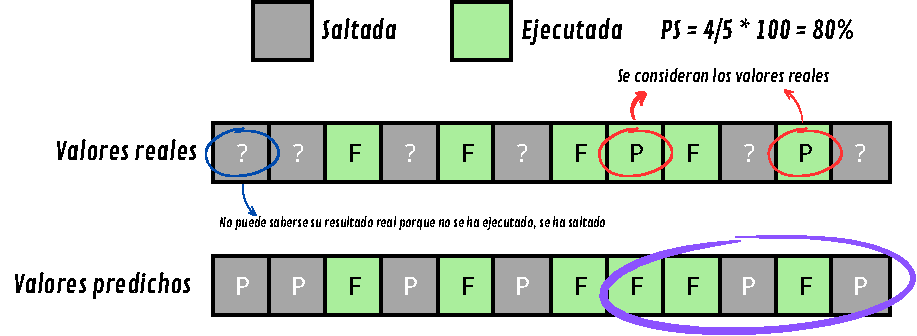
\includegraphics[scale=0.9]{images/PS.pdf}
    \caption{Cáculo del \textit{Performance Short}.}
    \label{fig:PS}
\end{figure}

\begin{figure}[H]
    \centering
    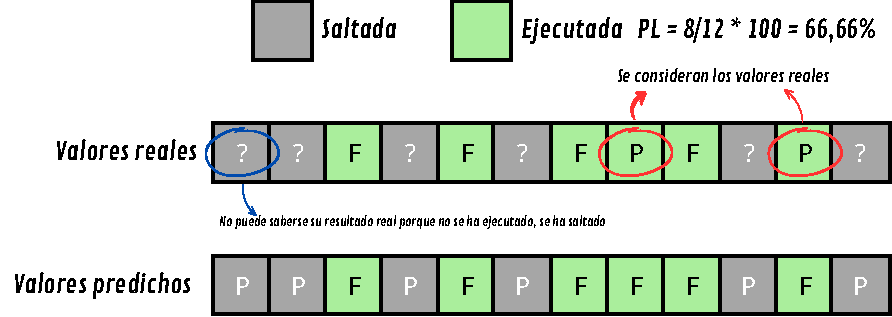
\includegraphics[scale=0.9]{images/PL.pdf}
    \caption{Cáculo del \textit{Performance Long}.}
    \label{fig:PL}
\end{figure}

\begin{figure}[H]
    \centering
    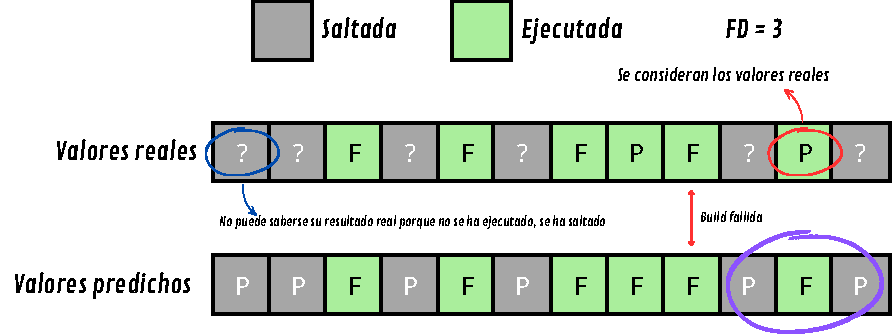
\includegraphics[scale=0.9]{images/FD.pdf}
    \caption{Cáculo del \textit{Failure Distance}.}
    \label{fig:FD}
\end{figure}

\subsection{Interfaz gráfica}
En nuestro proyecto, hemos implementado una interfaz gráfica simple que permite a los usuarios
interactuar con la aplicación de forma intuitiva y sencilla, reduciendo así la interacción a
bajo nivel con la aplicación. La interfaz se ha desarrollado con \textit{Angular}, un framework
de desarrollo de aplicaciones web desarrollado por \textit{Google}. La interfaz consta de dos
partes fundamentales, por un lado, un formulario que permite a los usuarios introducir la URL
de un repositorio concreto de \textit{GitHub} y la rama sobre la que desea predecir, y por otro
lado, una tabla que muestra los datos de cada uno de los repositorios indicando si se encuentran
disponibles sus modelos de predicción o no. \\

Cuando un usuario introduce la URL de un repositorio y la rama sobre la que desea predecir,
nuestra aplicación internamente realiza los siguientes pasos:

\begin{enumerate}
    \item Comprueba que la URL tiene un formato válido de acuerdo a las URLs de \textit{GitHub}.\\
    \item Comprueba si el repositorio y rama introducidos ya eran conocidos anteriormente por la
    aplicación. Si estos se encuentran en la base de datos, se devuelve un mensaje informativo y
    se detiene la ejecución. Si el repositorio no existe en la aplicación, se crea la estructura
    de directorios necesaria para el almacenamiento de los datos relativos a ese repositorio:
    \textit{builds}, \textit{features}, modelos, gráficos de evaluación, etc.\\
    \item Si se continúa con la ejecución, se procede a la extracción de las \textit{builds} del 
    repositorio.\\
    \item Una vez se han extraído las \textit{builds}, se procede automáticamente a la extracción
    de \textit{features} a partir de estas \textit{builds}.\\
    \item Finalmente, se procede de forma automática al entrenamiento de los modelos de acuerdo a
    las \textit{features} seleccionadas en nuestro enfoque. Esto genera unos modelos de predicción
    listos para predecir.\\
\end{enumerate}

Es importante mencionar que, todos los pasos anteriormente descritos se realizan de forma
asíncrona, es decir, el usuario no tiene que esperar a que se complete un paso para poder seguir
con el siguiente. Esto ofrece la posibilidad de introducir varios repositorios a analizar de
forma simultánea. Además, cuando se ha realizado la extracción de \textit{features}, el programa
genera automáticamente los modelos de predicción para todos los algoritmos de clasificación
estudiados en la Sección \ref{sec:model_construction}. Esto hace que el usuario no tenga que
preocuparse de seleccionar un algoritmo de clasificación en concreto, ya que la aplicación
automáticamente generará el modelo asociado.\\

\noindent A continuación, se muestra el formulario de entrada:

\begin{figure}[H]
    \centering
    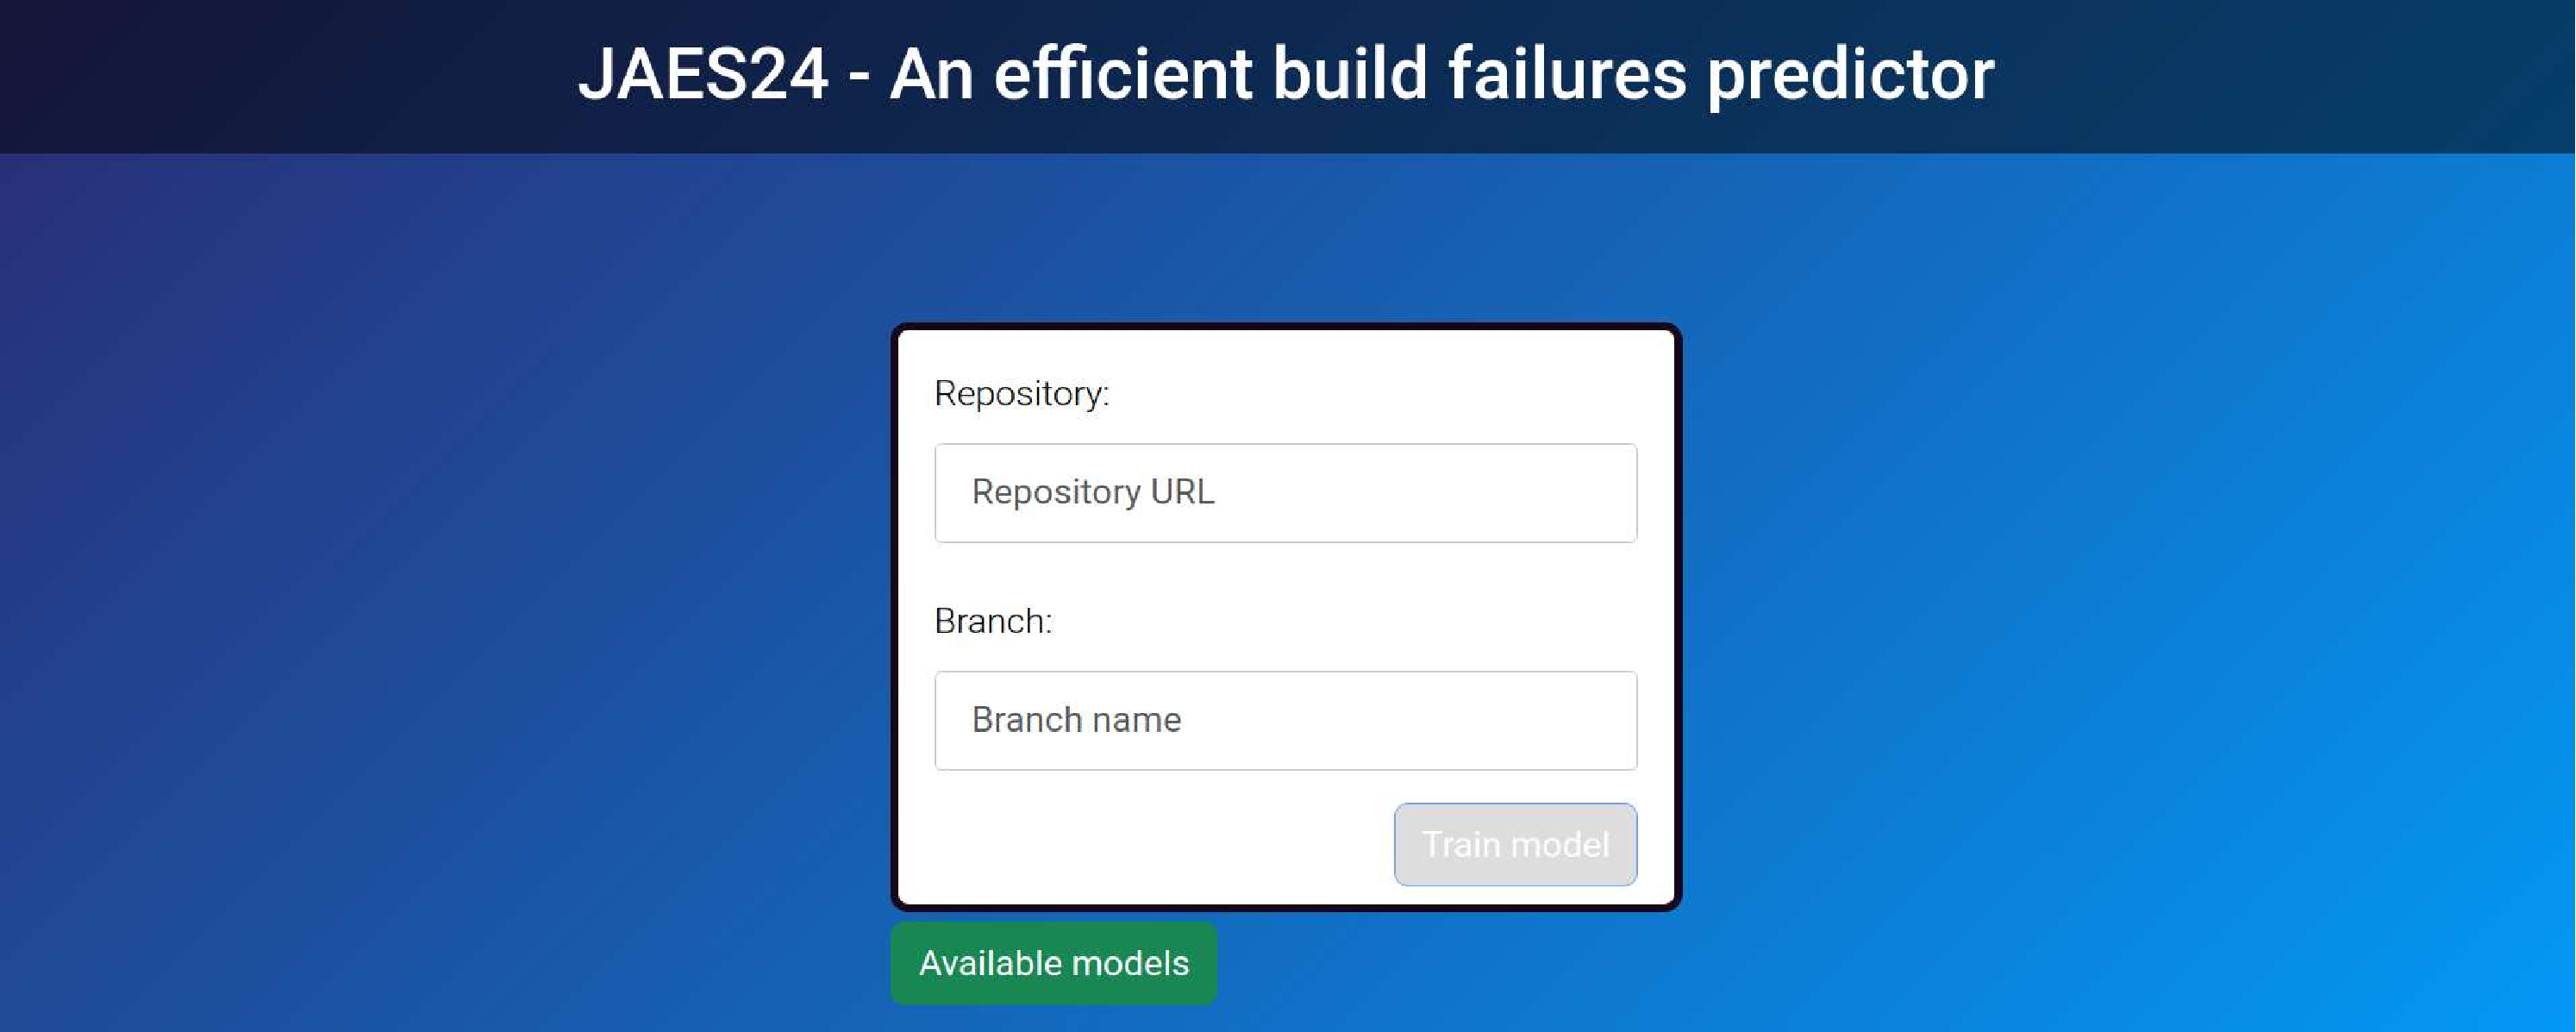
\includegraphics[scale=0.3]{images/input-form.pdf}
    \caption{Formulario de entrada.}
    \label{fig:input_form}
\end{figure}

Como es lógico, la extracción de las \textit{builds}, las \textit{features} y el entrenamiento
de los modelos, puede llevar un tiempo considerable. Este depende de la cantidad de \textit{builds}
a extraer y de la semántica de cada una de ellas, es decir, del tipo de evento que las origina
y la complejidad interna de cada una. No es similar extraer \textit{builds} originadas por un 
\textit{pull request}, que probablemente contenga mayor número de \textit{commits} y archivos 
modificados, que extraer \textit{builds} originadas por un \textit{push} simple. Por lo tanto,
se ha diseñado una pequeña tabla que recoge información sobre el estado de cada uno de los
repositorios introducidos. En ella, se muestra el nombre del repositorio, la rama sobre la que
se desea predecir, el archivo donde se almacenan las \textit{features} del repositorio, el
patrón del nombre que seguirán los modelos generados y, la última y más importante, si el modelo
se encuentra disponible o no.\\

\noindent A continuación, se muestra la tabla de repositorios:

\begin{figure}[H]
    \centering
    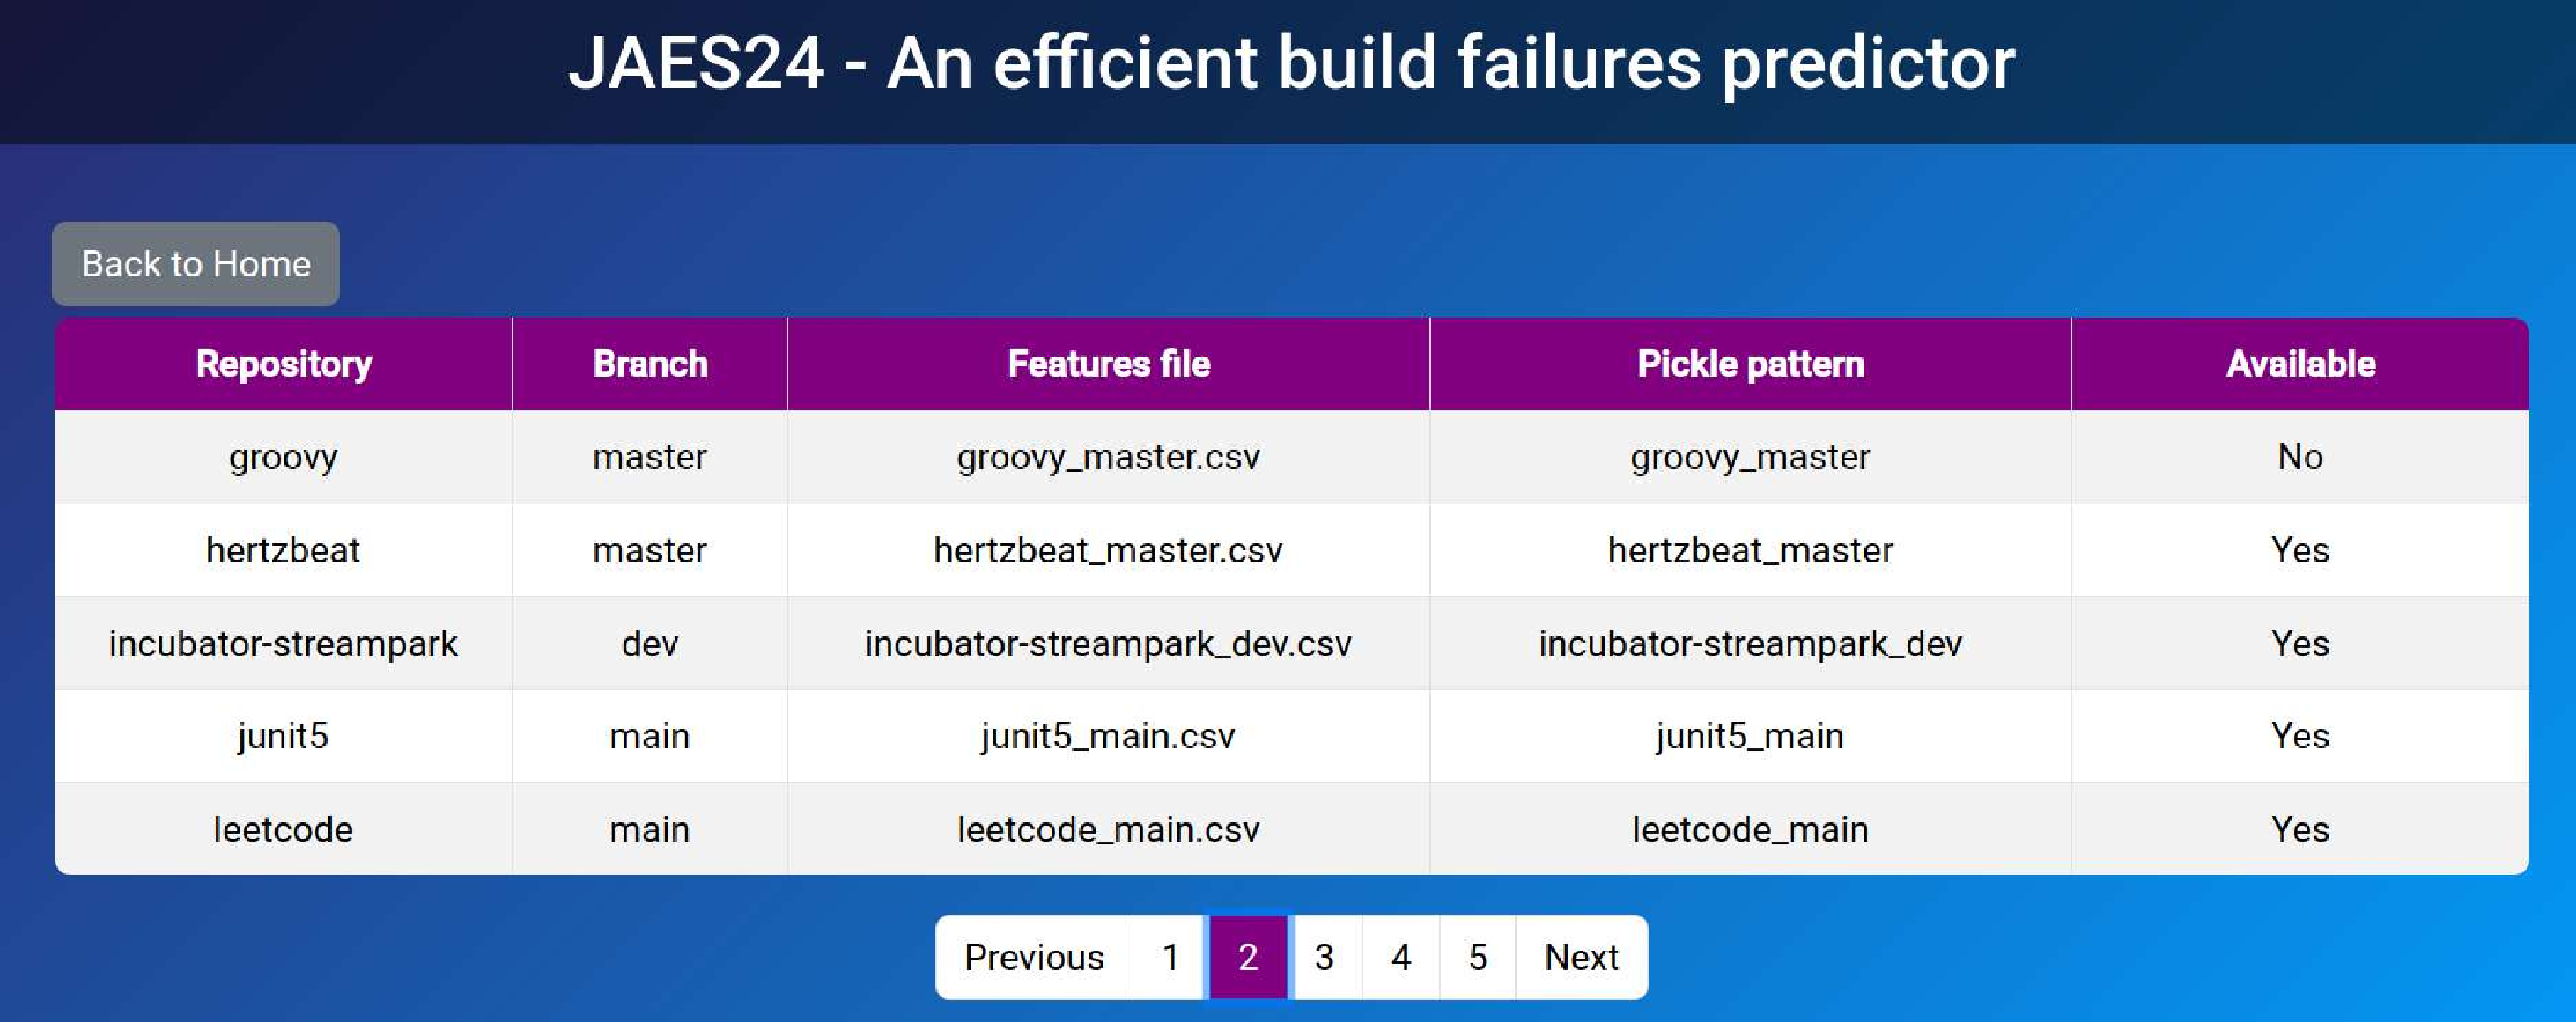
\includegraphics[scale=0.3]{images/available-models.pdf}
    \caption{Tabla de repositorios disponibles y el estado de sus modelos.}
    \label{fig:available_models}
\end{figure}

\subsection{Detalles técnicos de la implementación}
En esta sección, se muestran detalles técnicos de la implementación. Se explican las
tecnologías empleadas y las características que estas nos proporcionan para la resolución
de nuestro problema, los recursos que utilizamos para extraer las \textit{builds} de los
repositorios y, finalmente, cómo se realiza la extracción de las \textit{features} a partir de
estas \textit{builds}.

\subsubsection{Tecnologías empleadas.}
Para la resolución de nuestro problema, hemos decidido utilizar las siguientes tecnologías:

\begin{itemize}
    \item \textbf{\textit{Docker}}: es una plataforma de código abierto que nos permite crear, desplegar
    y ejecutar aplicaciones en contenedores. Los contenedores son entornos de ejecución que por
    lo general son ligeros y portátiles, conteniendo todo lo necesario para que una aplicación
    pueda ejecutarse. En nuestra implementación, hemos creado tres contenedores: uno para albergar
    la base de datos, otro para el servidor \textit{Flask} que contiene toda la lógica de nuestra
    aplicación y, por último, un contenedor para el cliente \textit{Angular} donde residirá la
    interfaz gráfica.\\

    \item \textbf{\textit{Docker Compose}}: es una herramienta que nos permite definir y ejecutar
    aplicaciones \textit{Docker} de múltiples contenedores. Nos permite orquestar la comunicación
    y ejecución de los contenedores de forma sencilla y eficiente. Para ello, se utiliza un archivo
    de configuración con extensión \textit{.yml} donde se definen los servicios, redes, puertos,
    variables de entorno, volúmenes que se van a utilizar, etc. Concretamente, se han definido
    tres servicios, uno para la aplicación \textit{Flask}, otro para \textit{Angular} y otro para
    la base de datos.\\

    \item \textbf{\textit{Flask}}: es un ``microframework'' de \textit{Python} para el desarrollo
    de aplicaciones web. Se ha elegido porque es bastante ligero y fácil de usar, lo que nos
    permite centrarnos en la lógica de la aplicación sin tener que preocuparnos de detalles de la
    configuración. Además, nos permite una fácil gestión de las dependencias, algo fundamental
    para el uso de librerías como \textit{Scikit-learn}, \textit{Pandas} o \textit{Matplotlib}.\\

    \item \textbf{\textit{Angular}}: es un framework de desarrollo de aplicaciones web desarrollado
    por \textit{Google}. Se ha elegido por su arquitectura modular y porque permite crear
    interfaces reutilizables.\\

    \item \textbf{\textit{PostgreSQL}}: es un sistema de gestión de bases de datos relacional
    (RDBMS) de código abierto. Se ha elegido por su fiabilidad, escalabilidadd y por ser muy
    eficiente en la gestión de grandes volúmenes de datos. En nuestro caso, únicamente se ha
    usado para almacenar los valores de aquellos repositorios que han sido introducidos en la
    aplicación.\\
\end{itemize}

\subsubsection{\textit{GitHub} REST API.}
La \textit{GitHub} REST API \cite{20} es una interfaz de programación de aplicaciones (API) que permite a
los desarrolladores interactuar de forma programática con los servicios de \textit{GitHub}. Esta
API da un soporte completo para realizar operaciones como:

\begin{itemize}
	\item \textbf{Gestión de repositorios}: crear, modificar y eliminar repositorios.\\
	\item \textbf{Administración de \textit{issues} y \textit{pull requests}}: crear, modificar, comentar
    y cerrar \textit{issues} o \textit{pull requests}.\\
	\item \textbf{Gestión de usuarios y organizaciones}: obtener información de usuarios, modificar
    ajustes de la cuenta, manejar miembros de organizaciones o 	equipos de trabajo, etc.\\
	\item \textbf{Automatización de flujos de trabajo}: permite la integración de \textit{GitHub} con otras
    aplicaciones y servicios, permitiendo lanzar flujos de trabajo de forma automática.
\end{itemize}


Todas estas operaciones, lógicamente, se podrán realizar siempre y cuando los usuarios estén
correctamente autenticados y tengan los permisos necesarios en relación con los recursos sobre los
que desea realizar la operación.\\

En nuestra solución, hemos realizado peticiones a esta API a través del uso de la librería
\textit{requests} de \textit{Python}. Esta nos proporciona todo lo necesario para realizar
peticiones HTTP de forma sencilla y eficiente. Además, para permitir un mayor número de peticiones
por minuto a esta API, hemos utilizado un \textit{token} de autenticación, que va incluido en la
cabecera de cada petición que realizamos.\\

\begin{table}[H]
    \centering
    \caption{\textit{\textit{\textit{Endpoints} de GitHub API REST usados}}.}
    \label{tab:API_endpoints}

    \begin{tabular}{|>{\centering\arraybackslash}m{11cm}|>{\centering\arraybackslash}m{5cm}|} % Encabezados centrados
        \hline
        \textbf{\textit{Endpoint}} & \textbf{Descripción} \\
        \hline
    \end{tabular}
    \begin{tabular}{|>{\raggedright\arraybackslash}m{11cm}|>{\raggedright\arraybackslash}m{5cm}|} % Contenido alineado a la izquierda en la esquina superior
        \hline
        \texttt{https://api.github.com/repos/OWNER/REPO/pulls} & Lista todos los \textit{pull requests} de un repositorio específico.\\
        \hline
        \texttt{https://api.github.com/repos/OWNER/REPO/pulls/PULL\_NUMBER} & Lista los detalles de un \textit{pull request} dado su identificador numérico.\\
        \hline
        \texttt{https://api.github.com/repos/OWNER/REPO/pulls/PULL\_NUMBER/commits} & Lista los \textit{commits} de un \textit{pull} request concreto.\\
        \hline
        \texttt{https://api.github.com/repos/OWNER/REPO/pulls/PULL\_NUMBER/files} & Lista los archivos modificados en un \textit{pull request} concreto.\\
        \hline         
        \texttt{https://api.github.com/repos/OWNER/REPO/actions/runs} & Lista todas las \textit{builds} ejecutadas en un repositorio.\\
        \hline
        \texttt{https://api.github.com/repos/OWNER/REPO/actions/runs/RUN\_ID} & Lista una \textit{build} específica dado su \textit{run id}.\\
        \hline
        \texttt{https://api.github.com/repos/OWNER/REPO/commits/COMMIT\_SHA} & Lista un \textit{commit} específico dado su valor SHA. \\
        \hline
        % Añade más filas según sea necesario
    \end{tabular}
\end{table}

En la Tabla \ref{tab:API_endpoints}, se muestran todos los \textit{endpoints} de la API de
\textit{GitHub} que hemos utilizado en nuestra implementación. Si nos fijamos, existen partes
en las urls que están marcadas con \texttt{OWNER}, \texttt{REPO}, \texttt{PULL\_NUMBER},
\texttt{RUN\_ID} y \texttt{COMMIT\_SHA}. Estos valores son parámetros que se deben sustituir por
los valores reales de los recursos sobre los que se quiere realizar la operación y que significan
lo siguiente: \texttt{OWNER}, nombre del propietario del repositorio, ya sea una persona o una
organización; \texttt{REPO}, nombre del repositorio del que se quiere obtener información;
\texttt{PULL\_NUMBER}, número identificador de un \textit{pull request}; \texttt{RUN\_ID},
identificador numérico de una \textit{build}; \texttt{COMMIT\_SHA}, valor SHA de un
\textit{commit}.\\

Obtener todas las \textit{builds} que se han ejecutado en un repositorio es una tarea que puede
parecer sencilla, ya que tenemos el quinto \textit{endpoint} que se muestra en la Tabla
\ref{tab:API_endpoints}, sin embargo, no es tan trivial como parece. Existen algunas restricciones
como el límite máximo de resultados que la API puede devolver, el número de peticiones por minuto
que se pueden realizar, la paginación de los resultados, etc., que hacen este proceso más
complejo. En nuestra implementación, se utiliza lo que se denomina un \textit{fine-grained
personal access token}, que nos permite aumentar el número de peticiones por minuto a la API.
Además, se ha implementado paginación para realizar las peticiones, ya que únicamente se pueden
obtener un máximo de $100$ \textit{builds} por página y, además, al llegar a un límite de $1000$
\textit{builds}, la API no permite obtener más \textit{builds} de forma directa. Finalmente, se
ha considerado la posibilidad de que \textit{GitHub} nos deniegue el acceso a la API por superar
el límite diario de peticiones, para lo cual guardamos el estado de ejecución del programa, para
reintentar pasado un tiempo definido la misma petición.

\subsubsection{Procesamiento de \textit{builds}.}
El procesamiento de las \textit{builds} es el paso en el que se extraen las \textit{features} de
cada una de las \textit{builds} extraídas en el paso anterior. Para ello, una vez las
\textit{builds} han sido extraídas del repositorio, estas se encuentran organizadas en un formato
JSON y por ficheros correspondientes a cada uno de los meses en los que se han ejecutado. Por
ejemplo, para un proyecto llamado \textit{junit5}, sus \textit{builds} quedarían organizadas de la
siguiente forma:

\begin{figure}[H]
    \centering
    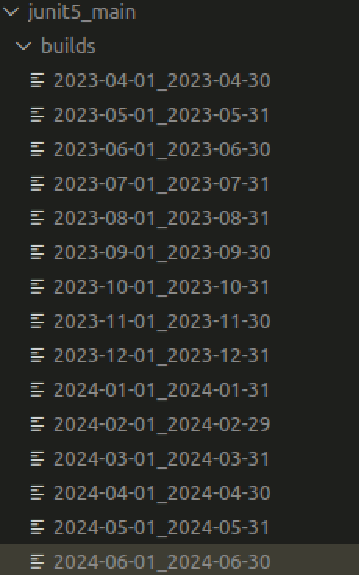
\includegraphics[scale=0.8]{images/Builds junit5.pdf}
    \caption{Organización de las \textit{builds} de un proyecto.}
    \label{fig:builds_junit5}
\end{figure}

Como vemos, por cada mes en el que se han ejecutado \textit{builds}, se ha creado un fichero
JSON conteniendo la información de todas las \textit{builds} ejecutadas en ese mes. Además, por
formato y organización, cada archivo está nombrado con el día de inicio y fin del mes concreto
al que pertenece.\\

A pesar de tener extraída la información de las \textit{builds}, muchos de los datos necesarios
para el cálculo de algunas \textit{features} no se encuentran disponibles directamente en la
información extraída. \textit{Features} como el  número de \textit{commits} (NC), el número de
archivos modificados (FC), el número de líneas de código modificadas (LC), el número de líneas de
código de \textit{test} modificadas (LT), el número de archivos añadidos (FA), el número de
archivos modificados (FM), el número de archivos eliminados (FR), el número de líneas de código
eliminadas (LR), el número de líneas de código añadidas (LA), si se han escrito pruebas unitarias
(UT) o el tiempo transcurrido entre \textit{commits} de una misma \textit{build} (CD), son
necesarias inferirlas a partir de la información que se tiene.\\
